\documentclass{standalone}
\usepackage{mintikz}

\usepackage{xfp}

\begin{document}
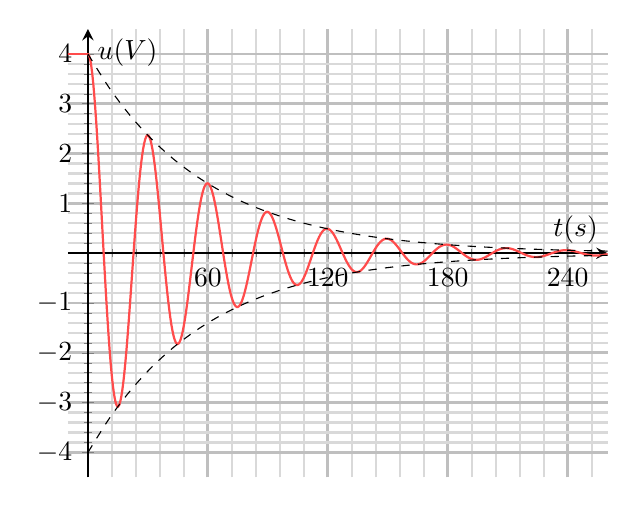
\begin{tikzpicture}
	\def\E{4}
	\def\R{793}
	\def\L{0.022639}
	\def\C{0.000000001}
	\def\Q{(1/\R)*sqrt(\L/\C)}
	\def\wo{sqrt(1/(\L*\C))}
	\def\w{\wo*sqrt(1-1/(4*\Q^2))}
	\def\T{2*3.1415/\w}
	\def\xmax{260e-6}
	\def\ymax{4.5}
	% \def\Q{14.66}
	% \def\wo{34100}
	% \def\w{\wo*sqrt(1-1/(4*\Q^2))}
	\begin{axis}[
			xmin=-1e-5, xmax=\xmax,
			ymin=-\ymax, ymax=\ymax,
			xlabel=$t(\si{\micro s})$, ylabel=$u(\si{V})$,
			axis lines=center,
			axis line style=thick,
			xtick={0,60e-6,...,300e-6},
			ytick={-4,...,4},
			scaled x ticks=base 10:6,
			/pgf/number format/sci subscript,
			xtick scale label code/.code={},
			% every x tick scale label/.style={at={(xticklabel cs:1)}, anchor=south},
			% ytick scale label code/.code={\pgfmathparse{int(-#1)}$y \cdot 10^{\pgfmathresult}$},
			% every y tick scale label/.style={at={(yticklabel cs:0.5)}, anchor = south, rotate = 90},
			grid=both,
			grid style={line width=.8pt, draw=gray!30},
			major grid style={line width=1pt, draw=gray!50},
			minor tick num=4,
			clip=false]
		% \draw[step=0.000001, color=gray!25] (-1e-4,-5) grid (\xmax,5);
		\addplot[thick,
			domain=-1e-5:0,
			samples=500,
			Red!70]
		{\E};
		\addplot[thick,
			domain=0:\xmax,
			samples=500,
			Red!70]
		{\E*exp(-(\wo*\x)/(2*\Q))*(cos(\w*\x r)+(\wo/(2*\Q*\w))*sin(\w*\x r))};
		\addplot[
			domain=0.0:\xmax,
			smooth, dashed,
			black]
		{\E*exp(-\wo*\x/(2*\Q))};
		\addplot[
			domain=0.0:\xmax,
			smooth, dashed,
			black]
		{-\E*exp(-\wo*\x/(2*\Q))};

		% \node[anchor=north east, align=right] (RQtext) at (axis cs: \xmax, \E.2) {
		% 	$R = \R\,\Omega$\\
		% 	$Q = \fpeval{round(\Q,2)}$\\
		% 	$T = \SI[scientific-notation=true]{\fpeval{round(\T,8)}}{s}$
		% };
		% \node[anchor=south east, align=right] (LCtext) at (axis cs: \xmax,-\E) {
		% 	$L = \num[scientific-notation=true]{\L}\,\rm H$\\
		% 	$C = \num[scientific-notation=true]{\C}\,\rm F$
		% };
	\end{axis}
\end{tikzpicture}
\end{document}
